% !TeX root = ../../main.tex
% !TeX spellcheck = en_US
% !TeX encoding = UTF-8

\chapter{Definitions}

	\section{Dynamical systems}
	% Dynamical systems, their properties and characteristics. Observable values and processes. Examples.
%	This book is conceived primarily to concentrate on processes of \gf\footnote{This term seemingly coined by Luckner and Schestakow \cite{luckner_simulation_1975} is, in author's opinion, best to describe the complex of phenomena and models connected with \gw dynamics}. However, the formalism used for the description of that class of phenomena is similar to that used in mathematical models pertaining to phenomena of different nature, decision was made to try to investigate problems arising from a more or less generalized point of view. This approach promises to create a more gentle introduction to the actual models in \gf proper.
%	
%	We start therefore with a few general definitions. Avoiding to go tofar, however, and trying not to touch deeper domains of pure philosophy, we will not try to formulate a definition for the basic concepts, such as \textbf{system}\index{system}, or \textbf{dynamical system}\index{dynamical system}, and will prefer a pragmatic approach instead. We refer the interested reader to classical works like \cite{Zadeh1963} and \cite{bossel_modeling_2018} that contain attempts to define them at the very fundamental level.

	Without trying to define the abstract concept of a system at a deeper philosophical level, in this treatise we rather prefer to remain on a more pragmatic basis and to use the notion intuitively. Therefore, instead of a definition there is rather a description of what a system is. It will be sufficient to specify its properties. Thus, a system is something which has a structure and behavior\footnote{Using the metaphor of the well-known "duck test" \cite{Duck_test_2026}, anything that has structure and behavior can be regarded as a system.}. If the state of a system does not change in time, the system is static. If there if temporal change, the system is dynamical. Static systems are outside of the topic if this treatise.
	
	Real-world systems, as well as their components, can be of natural (non-anthropogenic) or technological character, or include both kinds of components. The states and behavior of real-world systems can be observed or measured using defined conceptual state values (like the air temperature or a river discharge). Models of \dss differ from real-world systems in that they use modeled \textbf{state values} as abstractions of measured or observed ones. 
	
	A model is a partial description of a system, natural or technical, adapted for the ends of a concrete scientific or engineering study. 
	
	A model of a car as a \ds can include such values as the momentary velocity, distance from the starting point, acceleration, amount of fuel in the tank, battery voltage, luminosity of its rear lights, depending on what the model is pragmatically interested in for a concrete engineering study. 
	
	One and the same system can be however described by more than one model: if we are only interested in the mechanical properties of a car as a vehicle in space we will probably only include such characteristics as acceleration and velocity into our
	model, but not the battery voltage. If we are developing a hydraulic model of a river basin, we well probably not include water temperature and concentration of admixtures.
	
	In the following we will only speak of models of \dss, and of \textbf{state variables}, as the \textit{quid pro quo} of state values. For brevity, however, we will intermediately mix these concepts wherever it cannot come to confusion.
	
	Behavior of a \ds can be a result of their own inner instability, such as is the case with attractors of all kinds, but more often it is the result of external factors applied to the system. This case is also of a major practical significance, since we typically want to see which results an external action will produce in the system. Along with the state variables we will therefore consider the \textbf{external forces}, or inputs. 
	
	A \ds can be schematically represented by a scheme shown in Figure \ref{fig:abstractsystem}.
	\begin{figure}[H]
		\centering
		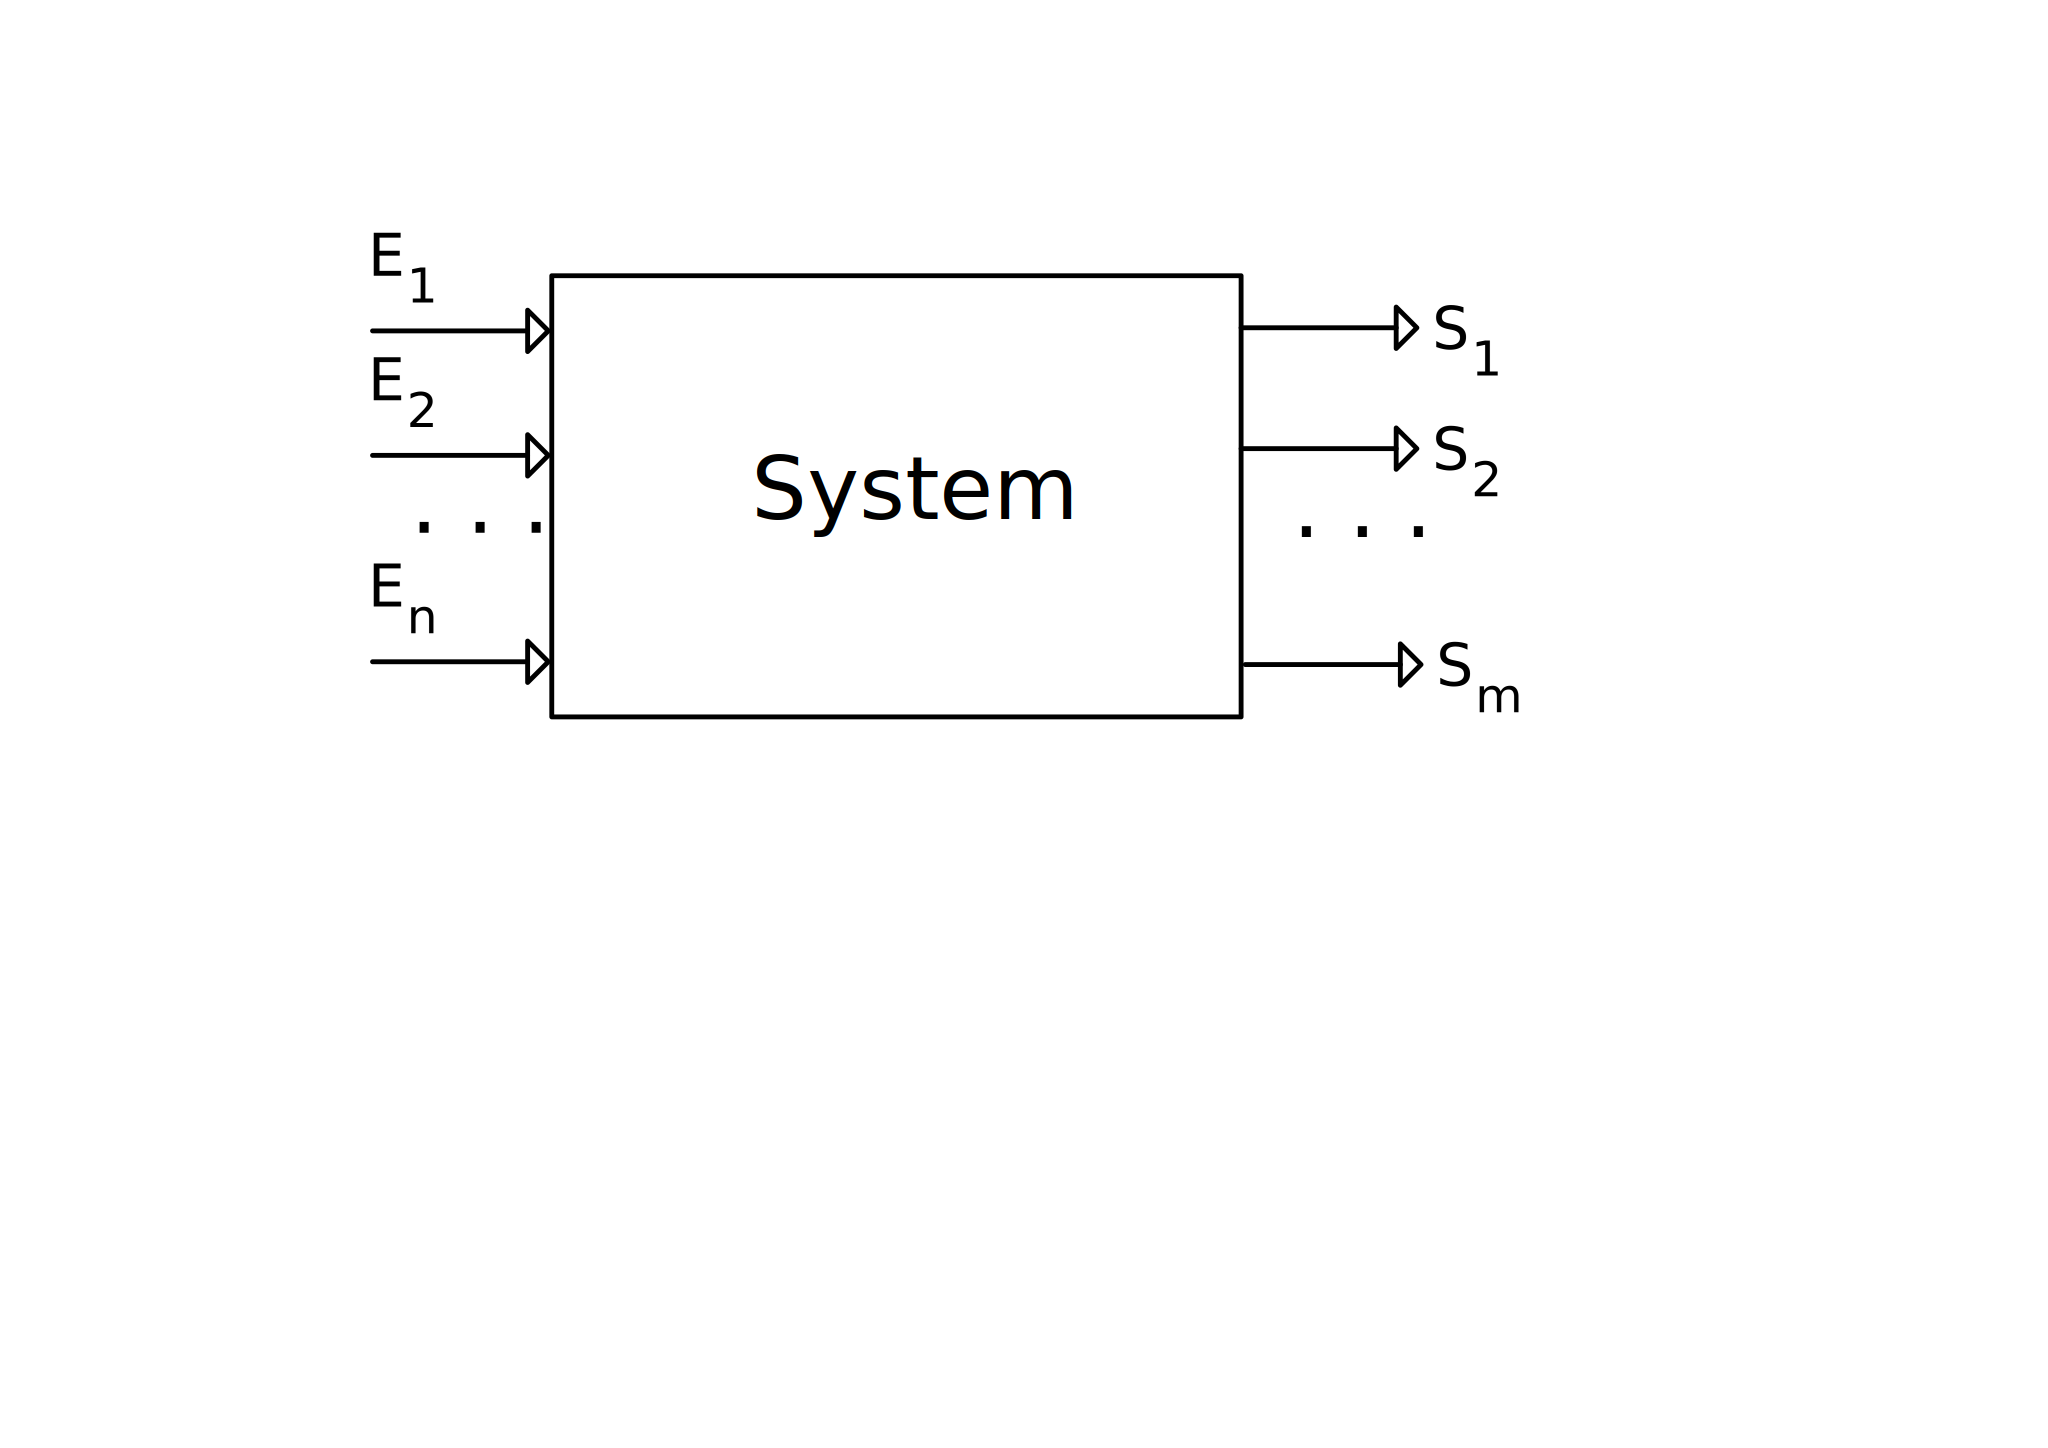
\includegraphics[width=0.5\linewidth]{abstract_system}
		\caption{Abstraction of a \ds. $E_1, ..., E_n$ are the external forces, $S_1, ..., S_m$ the state variables.}
		\label{fig:abstractsystem}
	\end{figure}
	
	\paragraph{"Black", "opaque", and "glass" boxes\\}
	Schematic depiction like that in Figure \ref{fig:abstractsystem} is sometimes called its "black-box" representation \cite{bossel_modeling_2018}. The inner details of a system are modeled with different states of certainty and precision. Some systems, such as electrical circuits can be modeled with a very high level of precision: in a known electrical scheme with known parameters all processes can be predicted to a very high level of accuracy -  they are the "glass" boxes. 
	
	On the other pole are systems that consider processes and phenomena that can be only observed by their external manifestations. For example, we can observe certain brain activities and even measure things like brain waves or neural patterns, but how the thinking - human thoughts arising from neural activity - takes place within the brain is a mystery. This is the case where the system is a "black box".
	
	\Gf systems, of which we will mostly speak in this treatise, take an intermediary place between "glass" and "black" boxes. The laws of \gw dynamic are well-known, as well as is known the concrete geological structure of the aquifers under consideration. However, this knowledge is never full: by no means, as in time of writing, is it possible to elucidate the complete pattern of the irregular distribution of filtration parameters and boundary conditions. \Gf models are "opaque". The same, thought to a lesser extent can be applied to some other systems including natural components, such as hydrological processes and river hydraulics.

	
	\section{Linear dynamical systems}
	% Section 1.2	Linear dynamical systems. Principle of superposition. Examples.
	Figure \ref{fig:abstractsystembasic} shows a simple model of a \ds containing one external force $E(t)$ and one state variable $S(t)$.
	
	\begin{figure}[H]
		\centering
		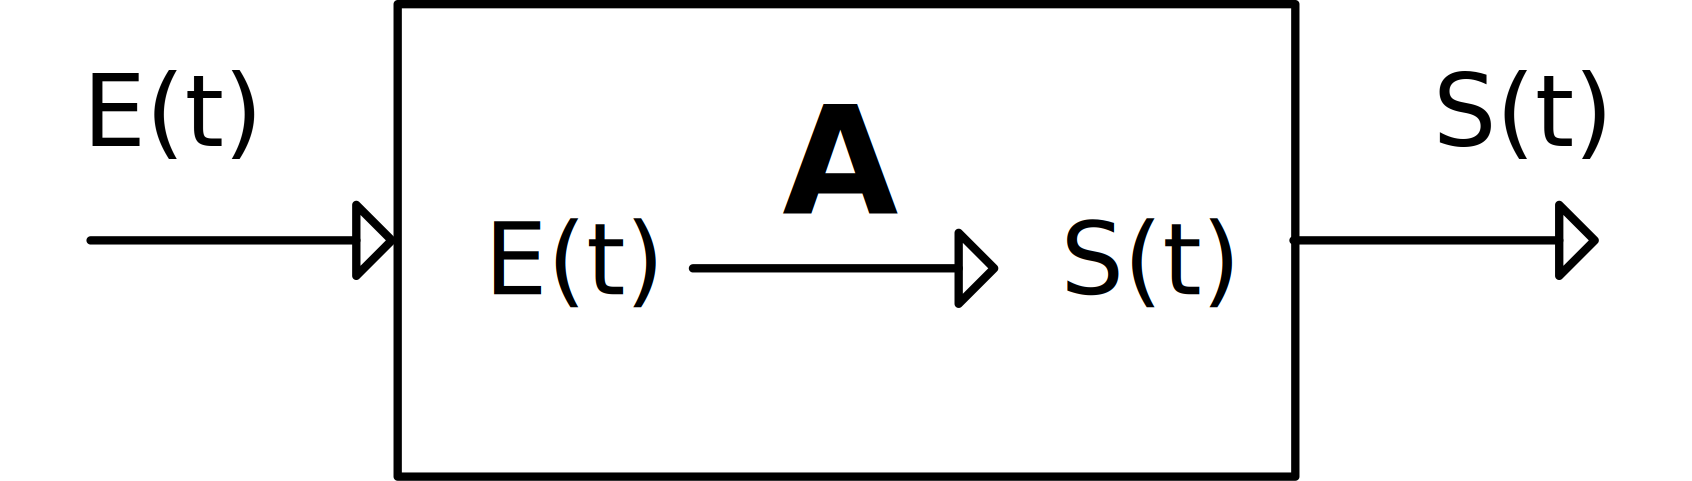
\includegraphics[width=0.5\linewidth]{abstract_system_basic}
		\caption{Simple \ds with one external force and one state variable}
		\label{fig:abstractsystembasic}
	\end{figure}
	
	That what happens within the system, which transforms the external force into the system variable, is formalized with an "A" above the arrow: $ E(t) \xrightarrow{A} S(t). $ This "A" stands for the "inner workings" of the system called its operator.
	
	The operator is, in other words, a mapping that converts external forces into state variables of the model, which can be mathematically formulated as 
	\begin{equation}
		S(t) = \mathbf{A} \circledast E(t),
	\end{equation}
	where the symbol $ \circledast$ is used to designate the action which the system applies to the external force to produce the output.
	
	\paragraph{Principle of superposition\\}
	Among all possible operators of system models like those shown in \ref{fig:abstractsystembasic} we are going now to select one special, but extremely important class, namely, linear operators.
	
	\section{Classification of linear dynamical systems}
	% Section 1.3	Classification of linear dynamical systems. Lumped and distributed systems. Examples.

% Example how to use \index
% Fourier transform\index{Fourier transform} \lipsum[1]


